%% Supplementary material of the IEEE TSP version (main.tex in this directory).
%% References with the prefix M- point to the main paper (package xr).
\documentclass[10pt]{article}
\usepackage[a4paper,margin=2.3cm]{geometry}
\usepackage{amsmath,amssymb,amsfonts,amsthm}
\usepackage{graphicx,booktabs,array,xcolor,xr}
\usepackage{algorithm}
\usepackage{algpseudocode}
\usepackage{cite}
\usepackage[hidelinks]{hyperref}
\externaldocument[M-]{main}
\graphicspath{{../paper/figs/}}
\newif\ifsp \spfalse
\newcommand{\mref}[1]{\ref{M-#1}}
\newcommand{\meqref}[1]{\eqref{M-#1}}
%% Macros and theorem environments shared by the SP (elsarticle) and TSP (IEEEtran) versions.
\newtheorem{theorem}{Theorem}
\newtheorem{proposition}{Proposition}
\newtheorem{lemma}{Lemma}
\newtheorem{corollary}{Corollary}
\theoremstyle{definition}
\newtheorem{definition}{Definition}
\newtheorem{remark}{Remark}

\newcommand{\Ts}{T_{\mathrm{s}}}
\newcommand{\cd}{c_{\mathrm{d}}}
\newcommand{\sd}{s_{\mathrm{d}}}
\newcommand{\ulo}{u_{\mathrm{lo}}}
\newcommand{\uhi}{u_{\mathrm{hi}}}
\newcommand{\xlo}{\xi_{\mathrm{lo}}}
\newcommand{\xhi}{\xi_{\mathrm{hi}}}
\newcommand{\gh}{\hat g}
\newcommand{\Hh}{\hat H}
\newcommand{\Op}[2]{{}^{\mathrm{#1}}\!\Delta^{#2}}
\newcommand{\WA}{W_{\mathrm A}}
\newcommand{\WB}{W_{\mathrm B}}
\newcommand{\WD}{W_{\mathrm D}}
\newcommand{\WE}{W_{\mathrm E}}
\newcommand{\Beta}{\mathrm{B}}
\newcommand{\eps}{\varepsilon}
\newcommand{\pending}[1]{\textcolor{red}{[#1]}}


%% References to labels of the main text: plain in the main text, prefixed M- in a supplement
\providecommand{\mref}[1]{\ref{#1}}
\providecommand{\meqref}[1]{\eqref{#1}}
%% Citation lists: the full list in the TSP version, a shorter one in the SP version (page limit)
\providecommand{\citesp}[2]{\ifsp\cite{#2}\else\cite{#1}\fi}

\newcommand{\partsdir}{../paper/parts/}
\newcommand{\tabfont}{\footnotesize}
\newcommand{\colfigwidth}{0.6\textwidth}
\renewcommand{\thesection}{S\arabic{section}}
\renewcommand{\thetable}{S\arabic{table}}
\renewcommand{\thefigure}{S\arabic{figure}}
\renewcommand{\theequation}{S\arabic{equation}}
\renewcommand{\theproposition}{S\arabic{proposition}}
\renewcommand{\theremark}{S\arabic{remark}}
\title{Supplementary Material for ``Variable-Order Fractional Operators from Fixed-Pole Banks: Definition by Structure, Error Guarantees, and Order Tracking''}
\author{}
\date{}
\begin{document}
\maketitle
\noindent Section, equation, table and figure numbers without the prefix S refer to the main paper. This supplement collects the continuous-time bank and results, state maps, the four types from one bank, the fixed-point realization and its board measurements, streaming multifractional Brownian motion, and two derivations.

%% Supplement shared by the SP version (paper/supplement.tex) and the TSP version (paper_tsp/supplement.tex).
%% References with the prefix M- point to the main text of the respective version (package xr).
\ifsp
%% Material that the SP version keeps out of its main text (page limit); the TSP version has it in the main text.
\input{\partsdir proofs}

\section{Related work: summary}\label{sup:related}
Table~\ref{tab:related} summarizes how the realizations reviewed in Sect.~\mref{sec:intro} treat a varying order.

\input{\partsdir tab_related}

\section{Design rule: term validation and holdout}\label{sup:rule}
Figure~\ref{fig:rule} shows the isolated error terms and the sealed holdout of Sect.~\mref{sec:results}.

\input{\partsdir fig_rule}

\section{Order tracking with a jump}\label{sup:tracking}
Figure~\ref{fig:tracking} shows the absolute error of the order in the ramp-and-jump scenario of Sect.~\mref{sec:track} (Table~\mref{tab:track}).

\input{\partsdir fig_tracking}

\section{Battery data: other realizations}\label{sup:battreal}
Table~\ref{tab:battreal} gives the numbers behind the comparison of realizations in Sect.~\mref{sec:battery}.

\input{\partsdir tab_battreal}
\fi

\section{Continuous-time bank}\label{sup:ctbank}
\paragraph{Diffusive representation.}

For $0<a<1$ and $S_a=\sin(\pi a)/\pi$~\cite{montseny1998,diethelm2023},
\begin{equation}
s^{-a}=S_a\int_0^\infty \frac{\xi^{-a}}{s+\xi}\,\mathrm d\xi,\qquad s^{a}=S_a\int_0^\infty \xi^{a-1}\,\frac{s}{s+\xi}\,\mathrm d\xi.\label{eq:diffusive}
\end{equation}
The order enters only through the density in $\xi$; the pole $-\xi$ of each element does not depend on it. This is the property the paper builds on.

\paragraph{Bank.} Let $\xi_k=\xlo e^{kh}$, $k=0,\dots,K-1$, be a geometric grid with spacing $h$ in $\ln\xi$, and apply the trapezoidal rule to~\eqref{eq:diffusive}. Every order is then written on the same bank of unit-DC-gain states $\dot x_k=-\xi_k x_k+\xi_k u$:
\begin{equation}
H_\alpha(s)=d(\alpha)+\sum_{k=0}^{K-1} m_k(\alpha)\,\frac{\xi_k}{s+\xi_k}.\label{eq:ctbank}
\end{equation}
For an integral, $\alpha=-a<0$, the weights are $m_k=hS_a\xi_k^{-a}$. For a derivative, $\alpha=a>0$, we use $s/(s+\xi)=1-\xi/(s+\xi)$: then $m_k=-v_k$ with $v_k=hS_a\xi_k^{a}$, and the feedthrough collects $\sum_k v_k$. The two truncated tails are closed by the geometric series of the virtual trapezoid nodes beyond the grid:
\begin{itemize}
\item one tail is lumped onto the outermost pole: $m_0\mathrel{+}=S_a\xlo^{-a}G_h(1-a)$ for integrals, $v_{K-1}\mathrel{+}=S_a\xhi^{a}G_h(1-a)$ for derivatives;
\item the other becomes feedthrough: $d=S_a\xhi^{-a}G_h(a)$ for integrals, $d=\sum_k v_k+S_a\xlo^{a}G_h(a)$ for derivatives.
\end{itemize}
Here
\begin{equation}
G_h(p)=\sum_{j\ge1}h\,e^{-pjh}=\frac{h}{e^{ph}-1},\qquad H_h(p,q)=G_h(p)-G_h(q).\label{eq:G}
\end{equation}
All nodes carry the full weight $h$. The bank therefore equals the infinite trapezoidal rule except for asymptotic tail residuals, and no $O(h^2)$ endpoint term appears. At $\alpha=0$ the bank is the identity ($m=0$, $d=1$). Since $S_aG_h(a)\to1$ as $a\to0$, the coefficients are continuous when the order crosses zero.

\paragraph{References for the experiments.}

For the continuous-time experiments we use the step responses of the A- and B-types. With $F(t,a)=t^{-a}/\Gamma(1-a)$, the step response of the constant-order operator $s^{a}$, they are
\begin{align}
y_{\mathrm A}(t) &= F\big(t,\alpha(t)\big), \label{eq:stepA}\\
y_{\mathrm B}(t) &= F\big(t,\alpha(0)\big)+\int_0^t \partial_a F\big(t-\tau,\alpha(\tau)\big)\,\dot\alpha(\tau)\,\mathrm d\tau. \label{eq:stepB}
\end{align}
Equation~\eqref{eq:stepB} is derived in Sect.~\ref{sup:stepB}. For a piecewise-constant order with switches at $T_i$, \eqref{eq:stepB} reduces to $F(t,\alpha_0)+\sum_i\big[F(t-T_i,\alpha_i)-F(t-T_i,\alpha_{i-1})\big]$.

\paragraph{Error terms.} The reasoning of Sect.~\ref{M-sec:design} applied to the diffusive representations gives the terms of Table~\ref{tab:ctterms}. The quadrature term is $2|\sin\pi a|e^{-\pi^2/h}$. The lower and upper tails exchange their forms between integrals and derivatives, as a consequence of the substitution $\xi\to1/\xi$ in~\eqref{eq:diffusive}.

\begin{table}[t]
\caption{Continuous-time error terms (relative frequency-response error on $\omega_1\le\omega\le\omega_2$), with $S=\sin(\pi a)/\pi$ and $G_h$, $H_h$ from~\eqref{eq:G}}\label{tab:ctterms}
\begin{tabular}{@{}lll@{}}
\toprule
Term & integral, $\alpha=-a<0$ & derivative, $\alpha=a>0$\\
\midrule
quadrature (first alias) & $2\sin(\pi a)\,e^{-\pi^2/h}$ & $2\sin(\pi a)\,e^{-\pi^2/h}$\\
lower tail & $S(\xlo/\omega_1)^{2-a}H_h(1-a,2-a)$ & $S(\xlo/\omega_1)^{1+a}G_h(1+a)$\\
upper tail & $S(\omega_2/\xhi)^{1+a}G_h(1+a)$ & $S(\omega_2/\xhi)^{2-a}H_h(1-a,2-a)$\\
\bottomrule
\end{tabular}
\end{table}
In continuous time the rule of Sect.~\ref{M-sec:design} takes $h=\pi^2/\ln(4\max_a|\sin\pi a|/\eps)$ in closed form, and the lower and upper tails give $\xlo/\omega_1$ and $\xhi$ by closed-form and monotone root conditions.

\section{Continuous-time switching results}\label{sup:ct}
\paragraph{Continuous time.} Figure~\ref{fig:definition} and Table~\ref{tab:e1} show a unit step with one order switch at $t=2$\,s, at equal state count. The fixed-pole bank with output schedule tracks the A-type and the one with input schedule tracks the B-type, with errors down to $10^{-4}$--$10^{-5}$. Before the switch, all realizations have similar errors ($10^{-3}$--$10^{-4}$), so the differences come from the switch. The hot-swapped parallel Oustaloup approaches the A-type only slowly. The cascade form tracks neither type: its error stays between 0.16 and 4.6 and does not decrease with $S$.

One negative result motivates the discrete-time bank. The continuous-time bank with input schedule fails for a smooth \emph{derivative} order (relative error about 12), because modes faster than $1/\Ts$ respond to every step of the sampled order.

\begin{figure}[t]
\centering
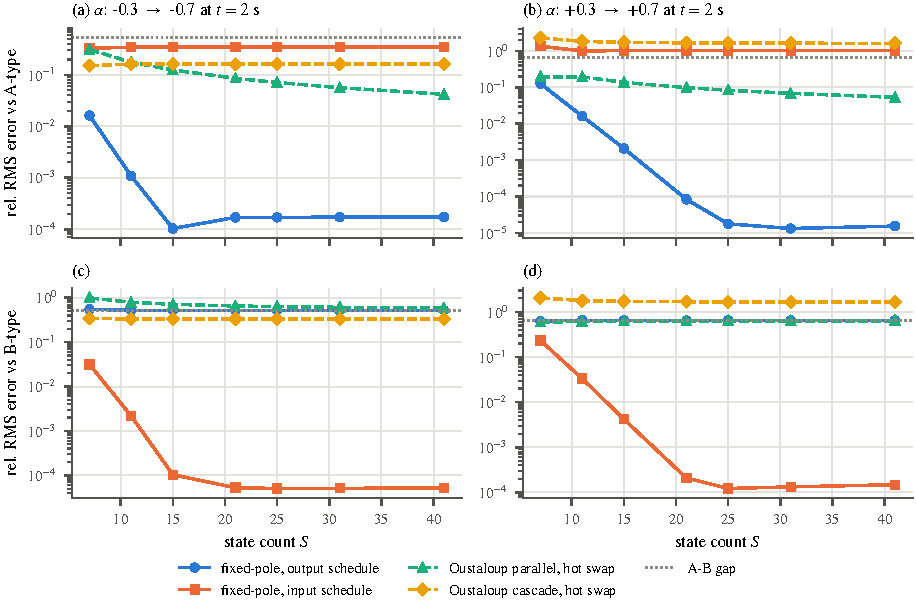
\includegraphics[width=\textwidth]{fig_definition.pdf}
\caption{Continuous time, unit step, one order switch at $t=2$\,s. Relative RMS error after the switch against the A-type (top) and B-type (bottom) closed forms versus state count. The dotted line is the distance between the two definitions. Every series has its own marker and line style}\label{fig:definition}
\end{figure}


Table~\ref{tab:e1} gives the numbers behind Fig.~\ref{fig:definition}.

\begin{table}[t]
\caption{Continuous time, step input: relative RMS error after a single switch. FP-out and FP-in are the fixed-pole bank with output and input schedule; Ou-par and Ou-cas are the hot-swapped Oustaloup forms. Arrows show $S=15\to41$; the cascade column is at $S=41$}\label{tab:e1}
\footnotesize\setlength{\tabcolsep}{4pt}
\begin{tabular}{@{}lccccc@{}}
\toprule
$\alpha_1\to\alpha_2$ & A--B gap & FP-out vs A & FP-in vs B & Ou-par vs A & Ou-cas, A / B\\
\midrule
$-0.3\to-0.7$ & 0.52 & $1.0\mathrm{e}{-4}\to1.7\mathrm{e}{-4}$ & $1.0\mathrm{e}{-4}\to5.1\mathrm{e}{-5}$ & $0.12\to0.042$ & 0.16 / 0.33\\
$+0.3\to+0.7$ & 0.65 & $2.1\mathrm{e}{-3}\to1.5\mathrm{e}{-5}$ & $4.2\mathrm{e}{-3}\to1.5\mathrm{e}{-4}$ & $0.14\to0.053$ & 1.6 / 1.7\\
$-0.5\to+0.5$ & 0.81 & $1.1\mathrm{e}{-3}\to4.3\mathrm{e}{-5}$ & $5.1\mathrm{e}{-4}\to3.1\mathrm{e}{-5}$ & $0.23\to0.085$ & 4.6 / 1.6\\
$+0.5\to-0.5$ & 1.35 & $9.8\mathrm{e}{-5}\to3.4\mathrm{e}{-5}$ & $9.4\mathrm{e}{-4}\to8.0\mathrm{e}{-6}$ & $0.25\to0.080$ & 0.24 / 0.87\\
\bottomrule
\end{tabular}
\par\smallskip{\footnotesize On the fixed band $[10^{-3},10^{5}]$\,rad/s used here, the fixed-pole bank reaches its tail floor near $S=15$. The rule of Sect.~\ref{M-sec:design} chooses the band from the tolerance instead.}
\end{table}



\section{State maps for moving-pole realizations}\label{sup:maps}
Theorem~\ref{M-thm:necessity} rules out exact maps, not approximate ones. A least-squares $\Phi$ fitted to an input ensemble can make the definitional error small in floating point , because the reachable states of both realizations concentrate in a low-dimensional subspace. Such a map, however:
\begin{itemize}
\item is dense, costing $S^2$ multiply-accumulates (MACs) at every switch;
\item is specific to each pair of orders, needing $2(P-1)$ maps for the $P-1$ neighbouring pairs of a grid of $P$ order levels;
\item depends on the statistics of the input.
\end{itemize}
State-update strategies for time-varying recursive filters suppress the transients of a coefficient change~\cite{zetterberg1988,valimaki1998}. By Theorem~\ref{M-thm:necessity}, no such update can make a moving-pole realization definition-consistent.




We fitted least-squares maps $\Phi$ for six single switches on mixed input ensembles and tested them on fresh inputs and on a unit step. In float64 the worst A-type definitional error fell from 0.14 (parallel form, hot swap) and $1.1\times10^4$ (cascade form) to below $10^{-6}$ at $S=31$. The map, however, is a dense $S\times S$ matrix with norm $10^3$ to $5\times10^4$, specific to each pair of orders. Rounded to 24 bits, it loses 3.5 to 4.3 orders of magnitude of accuracy in the parallel form and 7.4 to 9.1 in the cascade form ($S\ge21$). For the 1024 order levels of Sect.~\ref{M-sec:hw}, maps between neighbouring levels alone would need about 56\,Mbit, against 0.78--1.08\,Mbit for the whole coefficient table of the bank, which needs no map.



\paragraph{Setup.} For six single switches (at sample 2000, window 2000), we fitted $\Phi$ by truncated least squares on a mixed training ensemble of 4 classes with 200 inputs each (white, piecewise-constant, multisine, Brownian). We tested on fresh ensembles of 150 inputs per class and on a unit step, sweeping the truncation threshold. Besides the most accurate map, we report a robust \emph{minimum-norm} map: the map of smallest norm whose validation error is within twice the best. The maps were then rounded to float32 and to 24-bit fixed point.

\paragraph{Results.} Figure~\ref{fig:maps} and Table~\ref{tab:e2} report the worst case over the switches and the input classes. In float64 the error falls from $0.14$ (parallel, hot swap) and $1.1\times10^4$ (cascade, hot swap) to $1.7\times10^{-7}$ and $6.2\times10^{-7}$ at $S=31$. The map is, however, a dense $S\times S$ matrix, with norm between $10^3$ and $5\times10^4$ even for the minimum-norm choice. Rounded to 24 bits, the map loses 3.5 to 4.3 orders of magnitude of accuracy in the parallel form and 7.4 to 9.1 in the cascade form for $S\ge21$. In the cascade form the 24-bit error exceeds 1, and even float32 rounding raises it to $0.26$--$0.81$ for $S\ge15$.

With a smooth derivative order quantized to 41 levels (80 grid crossings, parallel form), a chain of maps reduced the step-input error from $4.1\times10^{-2}$ to $1.2\times10^{-4}$ ($S=15$). The fixed-pole bank needs no map, and its definitional error is exactly zero. For the $P=1024$ order levels of Sect.~\ref{M-sec:hw}, maps between neighbouring levels alone would need about 56\,Mbit of storage at $S=33$ and 25 bits per entry, against 0.78--1.08\,Mbit for the whole coefficient table of the bank.

\begin{figure}[t]
\centering
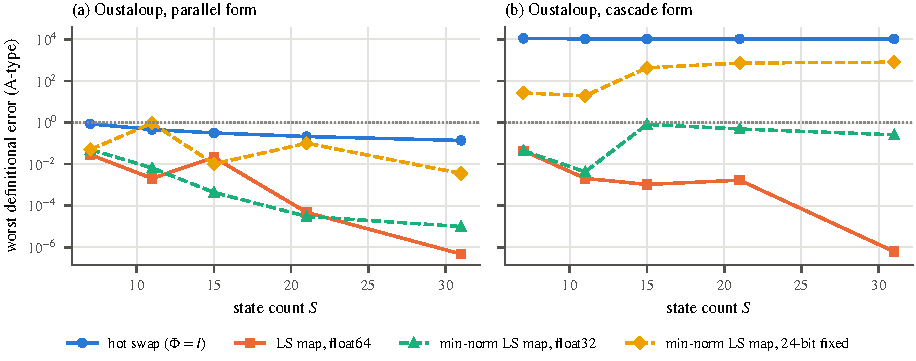
\includegraphics[width=\textwidth]{fig_maps.pdf}
\caption{Worst definitional error (A-type) after one switch, over six switches and five input classes including the step. Hot swap versus least-squares state maps in float64, and the minimum-norm map rounded to float32 and to 24-bit fixed point. The dotted line marks an error of 1}\label{fig:maps}
\end{figure}

\begin{table}[t]
\caption{State maps for the Oustaloup forms: worst A-type definitional error over 6 switches and 5 input classes (including the step), and the largest norm of the minimum-norm map}\label{tab:e2}
\footnotesize\setlength{\tabcolsep}{4pt}
\begin{tabular}{@{}llccccc@{}}
\toprule
 & & & & \multicolumn{3}{c}{minimum-norm map}\\
\cmidrule(l){5-7}
$S$ & form & hot swap & LS, float64 & float64 ($\|\Phi\|_2$) & float32 & 24-bit\\
\midrule
7  & parallel & 0.86 & $2.8\mathrm{e}{-2}$ & $5.0\mathrm{e}{-2}$ ($3\mathrm{e}{4}$) & $5.0\mathrm{e}{-2}$ & $5.0\mathrm{e}{-2}$\\
15 & parallel & 0.32 & $2.1\mathrm{e}{-2}$ & $4.4\mathrm{e}{-4}$ ($5\mathrm{e}{4}$) & $4.3\mathrm{e}{-4}$ & $1.0\mathrm{e}{-2}$\\
31 & parallel & 0.14 & $4.7\mathrm{e}{-7}$ & $1.7\mathrm{e}{-7}$ ($5\mathrm{e}{3}$) & $9.8\mathrm{e}{-6}$ & $3.6\mathrm{e}{-3}$\\
7  & cascade & $1.1\mathrm{e}{4}$ & $4.4\mathrm{e}{-2}$ & $4.4\mathrm{e}{-2}$ ($9\mathrm{e}{2}$) & $4.4\mathrm{e}{-2}$ & $2.7\mathrm{e}{1}$\\
15 & cascade & $1.1\mathrm{e}{4}$ & $1.0\mathrm{e}{-3}$ & $3.2\mathrm{e}{-4}$ ($8\mathrm{e}{3}$) & $8.1\mathrm{e}{-1}$ & $4.3\mathrm{e}{2}$\\
31 & cascade & $1.1\mathrm{e}{4}$ & $6.2\mathrm{e}{-7}$ & $6.2\mathrm{e}{-7}$ ($4\mathrm{e}{4}$) & $2.6\mathrm{e}{-1}$ & $8.1\mathrm{e}{2}$\\
\bottomrule
\end{tabular}
\par\smallskip{\footnotesize The fixed-point test rounds $\Phi$ to a single Q format; per-row scaling might do better. The fixed-pole bank needs $\Phi=I$ and has zero definitional error.}
\end{table}



\section{Which type does a hot swap implement?}\label{sup:hotswap}
Using the own-type references (definitional error) of Sect.~\ref{M-sec:results}, we asked which of the four types each hot-swapped realization is closest to, over 8 cases (four piecewise-constant order profiles, step and white-noise inputs) for $N=7$ and $N=15$:
\begin{itemize}
\item the fixed-pole bank is closest to A (output schedule) or B (input schedule) in all cases, at distances $\le2.1\times10^{-14}$;
\item the parallel Oustaloup form is closest to the A-type in all cases, at distances up to $0.42$;
\item for the cascade form with $\omega_h=10^3$\,rad/s, the closest type is A, B, D and E in two cases each, so the cascade has no consistent type; with $\omega_h=10^5$\,rad/s it is A or B, at distances up to $1.3\times10^{3}$;
\item with $\omega_h=10^5$\,rad/s, above the Nyquist frequency, the zero-order-hold members of the integral approximations have zeros outside the unit circle (moduli 3 to 41), and their own D- and E-types cannot even be formed in 6 of 8 cases.
\end{itemize}



\section{Four types from one bank}\label{sup:types}
\begin{remark}[VO relaxation equations]\label{rem:relax}
The same structure solves $\Op{T}{\alpha}y+\lambda y=u$ for $T\in\{\mathrm{A,B,D,E}\}$ at $O(K)$ per sample:
\begin{itemize}
\item A and B: $y_n=(u_n-\eta_n)/(\gh_0(\alpha_n)+\lambda)$;
\item D and E: write $y=\hat W(-\alpha)z$ with $z=u-\lambda y$, which gives $y_n=\big(\gh_0(-\alpha_n)u_n+\eta_n\big)/\big(1+\lambda\gh_0(-\alpha_n)\big)$, the bank being driven by $z_n=u_n-\lambda y_n$.
\end{itemize}
A direct triangular solve of the GL equations costs $O(N^2)$.
\end{remark}
\begin{remark}[Signs instead of eigenvalues]\label{rem:eig}
The dominant pole of a derivative-bank inverse lies extremely close to $z=1$, and general eigenvalue solvers are unreliable there. In one holdout design (order $0.95$, $K=35$), a 50-digit bisection places the dominant pole at $1-2.9\times10^{-12}$, while a double-precision eigenvalue routine reports modulus $1+4.5\times10^{-9}$. The signs of $\Hh(1)$ and $\Hh(-1)$, in contrast, are computed to full relative precision, and in fixed point they are evaluated exactly (Sect.~\ref{sup:hw}).
\end{remark}


\paragraph{Definitions.} The literal recursions~\eqref{M-eq:D},~\eqref{M-eq:E} agree with $\WA(-\alpha)^{-1}$ and $\WB(-\alpha)^{-1}$ to $1.4\times10^{-13}$. The dual compositions ($\mathrm A\circ\mathrm D$, $\mathrm D\circ\mathrm A$, $\mathrm B\circ\mathrm E$, $\mathrm E\circ\mathrm B$) return the identity to $10^{-12}$. The non-dual compositions (A$\circ$A, B$\circ$B, A$\circ$B, B$\circ$A, A$\circ$E, B$\circ$D, D$\circ$E, D$\circ$D) differ from the identity by $10^{-2}$ to $2.4\times10^{3}$.

\paragraph{Bank.} A bank designed for $\eps=10^{-5}$, $|\alpha|\le0.95$ and $R=4000$ ($K=41$) was run in all four types over 5 order profiles and 3 inputs (Table~\ref{tab:e4}). The error against the literal definitions is at most $6.9\times10^{-5}$. The definitional error is at rounding level, and the duality holds in the bank to $2\times10^{-14}$. The largest output errors occur for derivatives with smooth inputs, where the weights cancel (the bound~\eqref{M-eq:bound}).

\begin{table}[t]
\caption{One bank ($K=41$) in four types: error against the literal GL definitions (15 cases), and against the bank's own type (the 12 piecewise-constant cases)}\label{tab:e4}
\begin{tabular}{@{}lcc@{}}
\toprule
Type & vs literal definition & vs own type (definitional)\\
\midrule
A & $9.5\times10^{-8}$ to $6.9\times10^{-5}$ & $\le2.6\times10^{-14}$\\
B & $3.1\times10^{-8}$ to $1.2\times10^{-5}$ & $\le1.0\times10^{-14}$\\
D & $2.0\times10^{-8}$ to $6.5\times10^{-5}$ & $\le2.3\times10^{-14}$\\
E & $2.2\times10^{-8}$ to $5.5\times10^{-5}$ & $\le2.8\times10^{-13}$\\
\bottomrule
\end{tabular}
\end{table}

\paragraph{Inverse stability.} Over the 200 discrete-time holdout designs, checked at 25 orders spanning each design range, the inverse was stable at every order in 200/200 designs with the DC floor and in 101/200 without it. Figure~\ref{fig:types}b shows a D-type integral of order $0.95$ driven by white noise for $2\times10^5$ samples ($\eps=10^{-2}$, $R=1000$, $K=15$). Without the floor the output RMS grows to $1.9\times10^{21}$; with the floor it stays below $0.36$.

\paragraph{Relaxation equations.} For $\Op{T}{\alpha}y+\lambda y=u$ (Remark~\ref{rem:relax}; $K=40$, $n=4000$), the bank matched the triangular GL solutions to $1.7\times10^{-5}$ ($\lambda=1$) and $4.9\times10^{-7}$ ($\lambda=100$). The solutions of different types differed by up to $0.40$ for $\lambda=1$ (Fig.~\ref{fig:types}a), so the choice of type changes the solution visibly. For $\lambda=100$ the term $\lambda y$ dominates and the types differ by at most $0.02$.

\begin{figure}[t]
\centering
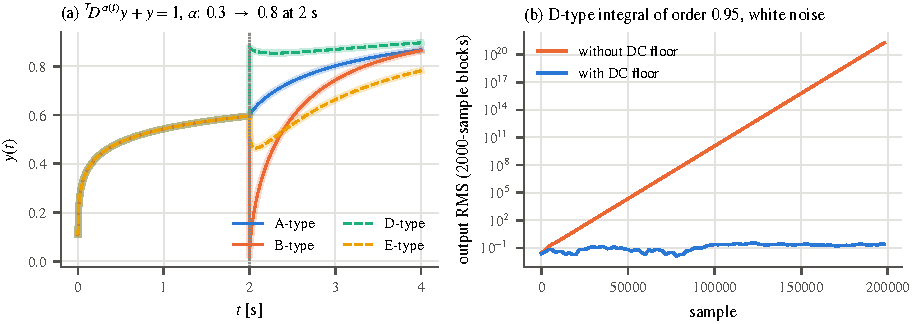
\includegraphics[width=\textwidth]{fig_types.pdf}
\caption{(a) Relaxation equation of all four types with one bank; thin lines are the bank, wide light lines the triangular GL solutions. (b) D-type integral of order 0.95 (inverse of the 0.95 derivative bank) on white noise, with and without the DC floor}\label{fig:types}
\end{figure}


\section{Fixed-point realization}\label{sup:hw}


The design point is $R=4000$, $\eps=10^{-4}$ and $|\alpha|\le0.95$, giving $K=32$ plus the delay mode. Orders come from a grid of $P=1024$ levels, $\alpha_i=0.95\,(2i/(P-1)-1)$, so $\Delta\alpha=1.9\times10^{-3}$.

\begin{algorithm}[t]
\caption{One sample of the bank, all four types. In hardware the coefficient row is a ROM word addressed by the order index (mirrored for D and E), so an order or type change costs nothing}\label{alg:core}
\begin{algorithmic}[1]
\Require type $T\in\{\mathrm{A,B,D,E}\}$, order $\alpha_n$, input $x_n$; states $s_0,\dots,s_{K-1},\sd$
\State $a\gets\alpha_n$ if $T\in\{\mathrm{A,B}\}$, else $a\gets-\alpha_n$; read $(\cd,c_0,\dots,c_{K-1})$ for order $a$
\If{$T\in\{\mathrm{A,D}\}$} \Comment{output schedule}
  \State $\eta\gets\cd\,\sd+\sum_k c_k s_k$
\Else \Comment{input schedule}
  \State $\eta\gets\sd+\sum_k s_k$
\EndIf
\If{$T\in\{\mathrm{A,B}\}$} $v\gets x_n$;\ \ $y_n\gets v+\eta$
\Else\ $v\gets x_n-\eta$;\ \ $y_n\gets v$ \Comment{no divider in sample units}
\EndIf
\If{$T\in\{\mathrm{A,D}\}$} $s_k\gets\theta_k s_k+v$;\ \ $\sd\gets v$
\Else\ $s_k\gets\theta_k s_k+c_k v$;\ \ $\sd\gets\cd v$
\EndIf
\end{algorithmic}
\end{algorithm}


 The design point is $R=4000$, $\eps=10^{-4}$ and $|\alpha|\le0.95$, giving $K=32$ plus the delay mode, and the orders come from a grid of $P=1024$ levels, $\alpha_i=0.95\,(2i/(P-1)-1)$.

\subsection*{Arithmetic in sample units}

The core runs in sample units ($\Ts=1$), where $\gh_0=1$ for every order. The inversion of Proposition~\ref{M-prop:inverse} then needs no divider: $v_n=x_n-\eta_n$. Physical units follow from one gain $\Ts^{-\alpha_n}$, applied at the output for the A- and E-types and at the input for the B- and D-types. This follows directly from~\eqref{M-eq:A}--\eqref{M-eq:E}; for the E-type, substitute $z_n=\Ts^{-\alpha_n}\zeta_n$.

The number formats are as follows:
\begin{itemize}
\item \emph{Signals:} $W_S$-bit two's complement with $F$ fractional bits.
\item \emph{States:} $W_{ST}=W_S+13$ bits. Each mode stores its state scaled by a power of two $2^{G_k}$ (one gain per schedule) so that its own bound uses the full word. Without this scaling, the input-scheduled slow modes lose their increments $c_kv_n$, which lie far below the signal LSB; the B- and E-type errors were then $2\times10^{-2}$ to $0.66$.
\item \emph{Coefficients:} a $W_M$-bit mantissa with a 7-bit shift.
\end{itemize}
Products are rounded as $\mathrm{mulsh}(a,M,S)=(aM+2^{S-1})\gg S$. Algorithm~\ref{alg:core} of the main paper gives one sample of the core in exact arithmetic; the bit-accurate golden model and the RTL use the same sequence with the formats above.



\subsection*{Dynamic range: two operating envelopes}

For $|x|\le1$ over $4000$ samples, the frozen-order $\ell_1$ bound on the output is $2696$. For the A-type this bound holds under any switching, because each output uses the weights of a single order; for the B-type the switching stress tests stayed within it. For the D- and E-types, switching from an integral to a derivative order drives the output to $2.2\times10^6$ under a DC input, 820 times the frozen-order bound. The new inverse acts on a history that has grown under the old order. This is the behaviour of the recursive definitions themselves, not an artefact of the bank. We therefore size two envelopes with a factor-two margin: 14 integer bits for the forward types only (A/B), and 24 integer bits for all four types (A/B/D/E).

\subsection*{Quantization and inverse stability}

Quantization can undo the DC floor. Coefficients and pole steps are dyadic rationals, so the signs of $\Hh_q(\pm1)$ of every quantized ROM row can be evaluated exactly in rational arithmetic, which we did. With the floating-point floor alone:
\begin{itemize}
\item in the A/B configuration, 64 of the 512 positive-order rows have $\Hh_q(1)\le0$, the worst having its dominant inverse pole at $1+4.8\times10^{-6}$ (e-folding time $2.1\times10^5$ samples);
\item in the A/B/D/E configuration, 51 of 512 rows have $\Hh_q(1)\le0$, the worst ($\alpha=0.855$) having its pole at $1+1.9\times10^{-9}$ (e-folding time $5.2\times10^{8}$ samples, about 9 minutes at 1\,MS/s).
\end{itemize}
$\Hh_q(-1)$ was positive in every row. The \emph{quantization-aware} DC floor raises the delay mantissa in LSB steps until $\Hh_q(1)$ is at least the floating-point value $\Hh(1)$. It brings both counts to zero without any measurable change in accuracy.

\subsection*{Word length}

We swept $W_S\in\{32,\dots,56\}$ and $W_M\in\{16,18,25,32\}$ (Fig.~\ref{fig:wordlength}). The test set comprised 3 order profiles (random piecewise, a new order every sample, a sign-changing switch), 3 inputs, and all types of the envelope. A configuration was accepted if, for every type, its error against the literal definition was at most the floating-point bank's error plus $0.1\eps$. The smallest accepted configurations were:
\begin{itemize}
\item A/B: $W_S/W_{ST}/W_M=36/49/16$;
\item A/B/D/E: $48/61/25$.
\end{itemize}
With an 18-bit mantissa the D- and E-types stall near $10^{-3}$, because the inversion is ill-conditioned: the low-frequency gain of a derivative bank is about $R^{-\alpha}$. The floating-point bank itself has D- and E-type output errors up to $6\times10^{-4}$ at this design point, although its weight error is $10^{-4}$. This is the cancellation effect noted after~\eqref{M-eq:bound}, amplified by the inversion.

\begin{figure}[t]
\centering
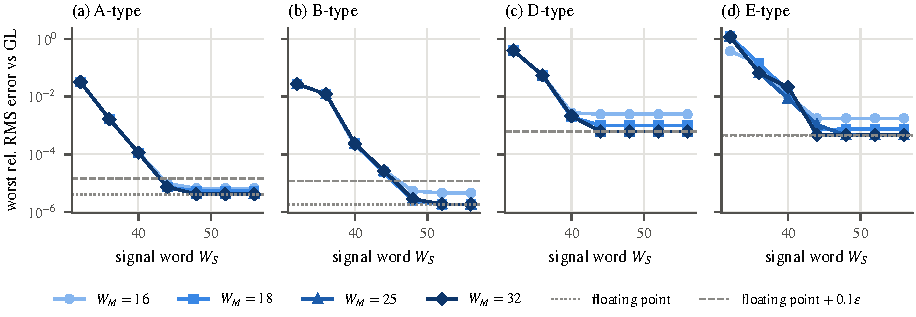
\includegraphics[width=\textwidth]{fig_wordlength.pdf}
\caption{Word length, A/B/D/E envelope: worst relative RMS error against the literal definitions versus signal word $W_S$ (state word $W_S+13$), for four mantissa widths. Dotted: floating-point bank; dashed: acceptance limit}\label{fig:wordlength}
\end{figure}




\paragraph{RTL, parity and resources.}

The core (\texttt{vo\_bank\_core.v}) is a non-pipelined, time-multiplexed state machine with synchronous coefficient, pole and gain ROMs. It produces one sample every $4K+7=135$ clock cycles. Order index and type are inputs with every sample. An order change only changes a ROM address: there is no reload and no extra cycle.

The test vectors cover constant, piecewise and per-sample orders, sign-changing switches, full-scale inputs, and type changes at run time. The type changes exercise the datapath; a type change is not itself a VO operation. Icarus Verilog and Vivado simulation matched the golden model bit for bit on all 94\,208 vectors (31\,744 for A/B, 62\,464 for A/B/D/E). Table~\ref{tab:rtl} gives the Vivado results for a Zynq-7020 (xc7z020clg400-1, Vivado 2026.1, out-of-context implementation of the core).

\begin{table}[t]
\caption{The two configurations on a Zynq-7020: resources and $f_{\max}$ of the core (Vivado, out of context), and bit-exact parity on the board (PYNQ-Z1). Sample rates are $f/135$}\label{tab:rtl}
\footnotesize\setlength{\tabcolsep}{3pt}
\begin{tabular}{@{}lccccccccc@{}}
\toprule
 & & \multicolumn{5}{c}{core, out of context} & \multicolumn{3}{c}{board}\\
\cmidrule(lr){3-7}\cmidrule(l){8-10}
Types & $W_S/W_{ST}/W_M$ & LUT & FF & DSP & BRAM & $f_{\max}$/MHz & clock/MHz & vectors (mism.) & MS/s\\
\midrule
A/B & 36/49/16 & 3\,214 & 1\,882 & 11 & 46 & 44.3 & 40.0 & 31\,744 (0) & 0.296\\
A/B/D/E & 48/61/25 & 4\,278 & 2\,337 & 15 & 64 & 39.3 & 34.5 & 62\,464 (0) & 0.255\\
\bottomrule
\end{tabular}
\end{table}

\paragraph{Board measurements.} Each configuration ran on a PYNQ-Z1 board behind an AXI4-Lite wrapper driven by the on-chip processor, with one reset and then all vectors in one stream. Both were bit-exact: the outputs were byte-identical to the simulation, with 0 mismatches (Table~\ref{tab:rtl}). A cycle counter confirmed 135 cycles from input acceptance to output and between back-to-back samples. The critical path runs from the coefficient ROM through the multipliers and the state adder in one cycle (43 logic levels for A/B/D/E); pipelining it would raise the clock.

For the long run, the D-type ran at the worst quantized row above ($\alpha=-0.855$, whose inverse is the derivative row of order $0.855$) on $2^{24}\approx1.7\times10^7$ samples of an on-chip 32-bit LFSR input with $|x|\le0.25$. The board kept, for every block of $2^{16}$ outputs, the maximum $|y|$, the sum of $y^2$ and a CRC-32. All 256 block records were identical to the golden model over the whole run. The golden model saw no overflow (peak state 51.3 of 61 bits, peak signal 29.4 of 48 bits), and the largest output, $|y|=85.7$, was far below full scale ($2^{24}$). The block RMS ranged from 2.1 to 79, as a fractional integral of order 0.855 of white noise wanders. This run shows bit-exactness and boundedness in hardware; it cannot by itself separate the two floors, because the floating-point floor's unstable pole would grow by only a factor of 1.03 over $2^{24}$ samples. Stability rests on the exact sign test above. The measurements were made with the new core; none is taken from~\cite{tcas_submission}.

%% =====================================================================
%% =====================================================================

\section{Streaming multifractional Brownian motion}\label{sup:mbm}


Multifractional Brownian motion lets the Hurst exponent vary in time~\cite{peltier1995}, and its definitions are in general not equivalent~\cite{stoev2006}. The Riemann--Liouville form (RL-mBm)~\cite{lim2001,muniandy2001} is a VO integral of white noise of order $H(t)+\tfrac12$, with the current order applied to the whole past. It is thus an A-type integral. Applying the order at the time each increment enters gives the B-type variant. Up to the discretization of the kernel and a per-increment factor $\sqrt{2H_j}\,\Gamma(H_j+\tfrac12)$, this is the memory-multifractional Brownian motion (MMFBM) of Wang et al.~\cite{wang2023mmfbm}, $X(t)=\int_0^t\sqrt{\alpha(s)}\,(t-s)^{(\alpha(s)-1)/2}\,\mathrm dB(s)$ with $\alpha=2H$. The input-scheduled bank applies that factor as a gain on each input sample. Other multifractional constructions treat a varying $H$ differently~\cite{surgailis2008,sly2007,ryvkina2015,slezak2023}; they are compared below. VO operators have been used to synthesize multifractional Gaussian noise before~\cite{sheng2011}, and simulation methods for mBm include~\cite{chan1998}.

In sample units, the discrete processes are
\[
X^{\mathrm A}_n=\sum_r g_r(-a_n)\,\xi_{n-r},\qquad X^{\mathrm B}_n=\sum_j g_{n-j}(-a_j)\,\xi_j,\qquad a_n=H_n+\tfrac12,
\]
with i.i.d.\ standard normal $\xi$. For $H>\tfrac12$ the order exceeds 1, outside the range of the bank. An integer integration can be split off exactly, but only in the right place:

\begin{proposition}[Integer split]\label{prop:split}
Let $\Sigma$ denote the cumulative sum. Then
\[
\Op{A}{-a}\xi=\Op{A}{-(a-1)}(\Sigma\xi),\qquad \Op{B}{-a}\xi=\Sigma\big(\Op{B}{-(a-1)}\xi\big).
\]
\end{proposition}
\begin{proof}
$(1-z^{-1})^{-a}=(1-z^{-1})^{-(a-1)}(1-z^{-1})^{-1}$ gives $w_m(-a)=\sum_{i=0}^{m}w_i(-(a-1))$ for every fixed $a$. For the A-type, apply this at the fixed order $a_n$ of output sample $n$ and exchange the sums. For the B-type, sample $j$ keeps its order $a_j$:
\[
\sum_{j\le n}\sum_{i\le n-j}w_i\big(-(a_j-1)\big)\xi_j=\sum_{m\le n}\sum_{j\le m}w_{m-j}\big(-(a_j-1)\big)\xi_j .
\]
The right-hand side is the cumulative sum of $\Op{B}{-(a-1)}\xi$.
\end{proof}

The reversed orders are not exact: the relative errors are 0.1 to 1.3 in our tests. With the split, one bank of order $\tfrac12-H$, which satisfies $|\tfrac12-H|<\tfrac12$, covers all of $0<H<1$. It crosses $H=\tfrac12$ seamlessly because the order $0$ is exact in the bank.

\paragraph{Results.} The bank was designed by the rule for $\eps=10^{-4}$ and $0.05\le H\le0.95$ ($K=22$ to 26 for $n=1024$ to 16\,384). Paths agree with the literal GL processes driven by the same noise to $1.9\times10^{-6}$ (A) and $2.4\times10^{-6}$ (B). Computed exactly from the weight matrix, the variance agrees with the exact formula to $3.1\times10^{-5}$ and the covariance to $1.7\times10^{-6}$. The local Hurst exponent, estimated by generalized quadratic variations~\cite{istas1997,coeurjolly2005}, follows a varying $H(t)$ with an RMSE of the mean of 0.014 to 0.036 for both types (Fig.~\ref{fig:mbm}). The bank needs 47 to 55 multiplications per sample, independent of $n$, against $n/2$ on average for the direct GL sum.

The two types differ sharply at a jump of $H$ from $0.3$ to $0.8$. The A-type variance jumps from 119 to $1.5\times10^5$, and the path is discontinuous: the squared increment at the jump is $1.3\times10^5$ times the typical one. The B-type is continuous, in line with the behaviour reported for MMFBM and incremental mBm~\cite{wang2023mmfbm,slezak2023}. Which definition to use is therefore a modelling decision with visible consequences~\cite{wang2023mmfbm}, and the bank makes either choice available at the same cost.

\begin{figure}[t]
\centering
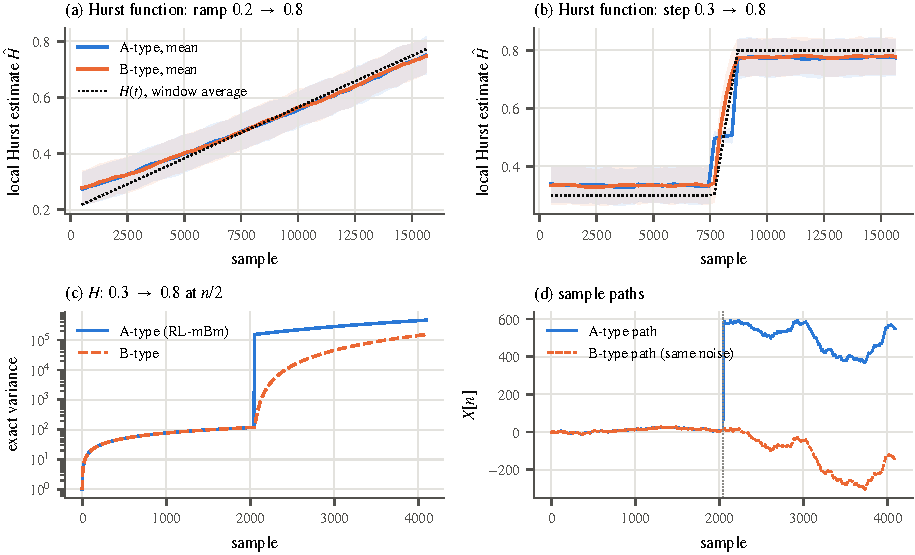
\includegraphics[width=\textwidth]{fig_mbm.pdf}
\caption{Streaming mBm. (a, b) Local Hurst estimates (mean $\pm$ one standard deviation over 400 paths) for a ramp and a step of $H$. (c) Exact variance of the A-type (RL-mBm) and B-type processes for a jump of $H$ at $n/2$. (d) Sample paths driven by the same noise}\label{fig:mbm}
\end{figure}

%% =====================================================================

\subsection*{Details}


Further alternatives to mBm treat a varying Hurst exponent differently. The incremental mBm of \'Sl\c{e}zak and Metzler~\cite{slezak2023} is defined through the covariance of its increments and shares the property that a change of $H$ acts only on new increments. Other alternatives to mBm include:
\begin{itemize}
\item the multifractional processes of Surgailis, built by nonhomogeneous fractional integration of white noise~\cite{surgailis2008}, whose covariance is not a local function of $H(t)$ and $H(t')$ as it is for mBm~\cite{bardet2013};
\item the integrated fractional white noise of Sly, proposed to avoid the extreme changes in magnitude of mBm~\cite{sly2007}.
\end{itemize}
Conversely, the variable-Hurst fBm of Ryvkina uses the current Hurst value in its kernel and has discontinuous paths wherever $H$ jumps~\cite{ryvkina2015}, like the A-type. VO operators have been used to synthesize multifractional Gaussian noise before~\cite{sheng2011}, and simulation methods for mBm include~\cite{chan1998}. Exact methods for stationary Gaussian processes such as circulant embedding~\cite{wood1994} rely on stationarity and do not apply directly when $H$ varies.

\paragraph{Further results.} Table~\ref{tab:mbm} and Fig.~\ref{fig:mbm} summarize the results. The bank was designed by the rule for $\eps=10^{-4}$ and $0.05\le H\le0.95$, giving $K=22$, 24 and 26 for $n=1024$, 4096 and 16\,384.

Second-order statistics were computed exactly, without Monte Carlo, from the $n\times n$ weight matrix of the generator. The variance agreed with the exact formula to $3.1\times10^{-5}$ and the covariance to $1.7\times10^{-6}$.

The local Hurst exponent was estimated by generalized quadratic variations~\cite{istas1997,coeurjolly2005}; see also~\cite{bardet2013}. For constant $H$ the estimator itself has a bias of $+0.06$ at $H=0.2$ and a standard deviation of $0.06$ (window 1024). For varying $H$ its mean followed $H(t)$ with RMSE $0.014$ to $0.036$, equally for both types.

The two types differ sharply at a jump of $H$ from $0.3$ to $0.8$. The A-type variance jumps from 119 to $1.5\times10^5$, and the path is discontinuous: the squared increment at the jump is $1.3\times10^5$ times the typical one. The B-type is continuous (ratio 1.0), in line with the behaviour reported for MMFBM and incremental mBm~\cite{wang2023mmfbm,slezak2023}. Which definition to use is therefore a modelling decision with visible consequences, as also argued in~\cite{wang2023mmfbm}. The bank makes either choice available at the same cost.

\begin{table}[t]
\caption{Streaming mBm with the fixed-pole bank}\label{tab:mbm}
\small
\begin{tabular}{@{}>{\raggedright\arraybackslash}p{0.44\textwidth}>{\raggedright\arraybackslash}p{0.52\textwidth}@{}}
\toprule
Quantity & Result\\
\midrule
integer split, correct order (A first, B last) & $\le9\times10^{-15}$\\
integer split, reversed order & $0.1$ to $1.3$\\
path vs literal GL, same noise & A $\le1.9\times10^{-6}$, B $\le2.4\times10^{-6}$\\
exact variance / covariance ($n=2048$) & $\le3.1\times10^{-5}$ / $\le1.7\times10^{-6}$ (Frobenius)\\
local Hurst tracking, varying $H$ (400 paths) & RMSE of mean 0.014 to 0.036, A and B alike\\
variance before/after a jump of $H$ from $0.3$ to $0.8$ & A $119\to1.5\times10^{5}$; B $119\to119$\\
cost per sample & bank 47 to 55 MACs ($n$-independent); direct GL $n/2$ on average\\
fixed-point core A/B (36/49/16), vs float & A $1.8\times10^{-5}$, B $8.9\times10^{-4}$\\
fixed-point core A/B/D/E (48/61/25), vs float & A $3.8\times10^{-6}$, B $1.2\times10^{-4}$\\
\bottomrule
\end{tabular}
\end{table}

\paragraph{Hardware.} The cores of Sect.~\ref{M-sec:hw} generate the same processes bit-exactly from integer noise. For the A-type, the accumulator sits in front of the core and is exact (an integer sum), so the small A/B core suffices. For the B-type, the accumulator follows the core and integrates its low-frequency rounding errors. The B-type therefore benefits from the wider configuration (Table~\ref{tab:mbm}, last two rows). Input scales were $2^{-9}$ for A and $0.25$ for B, chosen to keep the accumulated A-type input within the signal range.




\section{B-type step response}\label{sup:stepB}

The B-type operator in continuous time processes each input sample with the kernel of its entry order: $y(t)=\int_0^t K(t-\tau,\alpha(\tau))u(\tau)\,\mathrm d\tau$ with $K(s,a)=\partial_sF(s,a)=s^{-a-1}/\Gamma(-a)$, taken in the finite-part sense for $a>0$. For $u=1$, let $G(\tau)=F(t-\tau,\alpha(\tau))$. Then
\[
\frac{\mathrm dG}{\mathrm d\tau}=-\partial_sF(t-\tau,\alpha(\tau))+\partial_aF(t-\tau,\alpha(\tau))\,\dot\alpha(\tau),
\]
so $y(t)=G(0)-G(t)+\int_0^t\partial_aF\,\dot\alpha\,\mathrm d\tau$. The finite part removes $G(t)=F(0^+,\alpha(t))$, and $G(0)=F(t,\alpha(0))$. This gives~\eqref{eq:stepB}. For a piecewise-constant order, $\dot\alpha$ is a sum of Dirac impulses and the integral becomes the stated finite sum. In the experiments the smooth case was evaluated by adaptive quadrature after the substitution $s=v^m$ with $m(1-\alpha_{\max})\ge2$, which removes the weak singularity at $s=0$.


\section{Large-lag alias term}\label{sup:alias}

For large $r$ the integrand of~\eqref{M-eq:betax} is concentrated at $u=O(1/r)$, where $(1-e^{-u})^a\approx u^a$. Hence $f(x)\approx e^{(1+a)x}e^{-\rho e^x}$ with $\rho=r-a$. Its Fourier transform is $\hat f(\omega)=\Gamma(1+a-\mathrm i\omega)\rho^{-(1+a-\mathrm i\omega)}$, and $\hat f(0)=\Gamma(1+a)\rho^{-(1+a)}$ is the integral itself. The relative error of the infinite trapezoidal rule is $\sum_{k\neq0}\hat f(2\pi k/h)/\hat f(0)$, dominated by $k=\pm1$. Stirling's formula, $|\Gamma(1+a-\mathrm i\omega)|\sim\sqrt{2\pi}\,\omega^{a+1/2}e^{-\pi\omega/2}$, at $\omega=2\pi/h$ gives~\eqref{M-eq:Eq}. The result does not depend on $r$, which justifies the name large-lag term.


\bibliographystyle{IEEEtran}
\bibliography{../paper/refs}
\end{document}
